\section*{\nr.2 \tittwo (10 Punkte)}
\begin{enumerate}[(a)]
\item 
Im homogenen Magnetfeld werden die Ionen in der Draufsicht auf eine Kreisbahn gezwängt, da die Lorentzkraft senkrecht auf der Bewegungsrichtung der Ionen steht und so die hierfür notwendige Zentripetalkraft aufbringt. Für $\alpha=0$ ist die beschriebene Bahn genau ein Halbkreis, wie in \vref{fig:Massenspektrometer} dargestellt.
\begin{figure}[htbp]
\centering
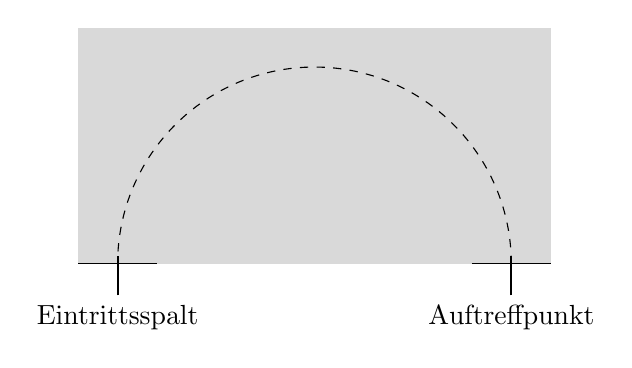
\begin{tikzpicture}
\fill[gray!30] (0,0) rectangle (6,3);
\draw (0,0) -- (1,0);
\draw[thick] (0.5,-0.4)node[below]{Eintrittsspalt} -- (0.5,0.1);
\draw[thick] (5.5,-0.4)node[below]{Auftreffpunkt} -- (5.5,0.1);
\draw (5,0) -- (6,0);
\draw[dashed] (5.5,0) arc[radius=2.5cm,start angle=0,end angle=180];
\end{tikzpicture}
\caption{Flugbahn der Ionen im Massenspektrometer}
\label{fig:Massenspektrometer}
\end{figure}

\item Die Lorentzkraft bringt die Zentripetalkraft für eine Kreisbewegung auf. Für den Betrag der Lorentzkraft gilt $F=qv_0B$, da das Magnetfeld senkrecht auf der Bewegungsrichtung steht. Also folgt:
\begin{equation}
\frac{mv_0^2}{r} = q v_0 B \iff r = \frac{mv_0}{qB}
\end{equation}
Die Eintrittsgeschwindigkeit erhält man aus der Überlegung, dass die Ionen durch die Beschleunigungsspannung $U_B$ von null auf die Geschwindigkeit $v_0$ beschleunigt werden:
\begin{equation}
qU_B = \frac{1}{2} m v_0^2 \implies v_0 = \sqrt{\frac{2qU_B}{m}}
\end{equation}

Der gesuchte Abstand ergibt sich aus dem doppelten Radius $r$:
\begin{equation}
x=2r = \frac{2mv_0}{qB} = \frac{2}{B} \sqrt{\frac{2mU_B}{q}}
\end{equation}

Eine Umformung nach $U_B$ ergibt:
\begin{equation}
U_B = \frac{q}{8m} B^2 x^2 \approx \SI{402}{\volt},
\end{equation}
wobei man die Masse von C-12 dadurch erhält, dass man seine molare Masse durch die Avogadro-Konstante teilt.

\item 
Der neue Abstand $x'$ zwischen Auftreffpunkt und Eintrittsspalt ergibt sich durch
\begin{equation}
x' = 2r \cos{\alpha} = x\cos{\alpha},
\end{equation}
wie man leicht aus dem gleichschenkligen Dreieck in \vref{fig:Divergenz} herleiten kann. Bemerkenswert ist, dass diese Formel sowohl für positive wie auch für negative $\alpha$ gilt.
\begin{figure}[htbp]
\centering
\begin{tikzpicture}[>={Stealth}]

%Die beiden Kreise
\draw[dotted] (3,0) circle[radius=3cm];
\draw (-1,0) -- (7,0);
\draw (0,0) -- ++(330:3cm) circle[radius=3cm] -- ++(30:3cm) --(0,0);

%Dreieck mit Beschriftungen
\begin{scope}[orange!90!black]
\node at (345:0.7cm){$\alpha$};
\path (330:3cm) ++ (30:3cm) ++(195:0.7cm)node{$\alpha$};
\draw[thick] (0,0) --node[below]{$r$} ++(330:3cm) --node[below]{$r$} ++(30:3cm) --node[above]{$x'$} cycle;
\draw (330:1cm) arc[radius=1cm,start angle=330,end angle=360];
\draw (330:3cm) ++ (30:3cm) ++(-1,0) arc[radius=1cm,start angle=180,end angle=210];

%"Drehtangenten"
\draw[dashed] (0,0) -- (0,2);
\draw[dashed] (0,0) -- (60:2);
\draw[dashed,<-] (60:1cm) arc[radius=1cm,start angle=60,end angle=90];
\node at (75:0.7cm){$\alpha$};
\draw[dashed,<-] (330:3cm) arc[radius=3cm,start angle=330,end angle=360];
\end{scope}

\end{tikzpicture}
\caption{Geometriebetrachtungen bei vorhandener Divergenz}
\label{fig:Divergenz}
\end{figure}

Aus $\Delta x = x- x'$ folgt dann direkt:
\begin{equation}
\cos{\alpha_\text{max}} = \frac{x-\Delta x}{x}
\end{equation}
Für die gegebenen Zahlenwerte folgt $\alpha_\text{max}\approx \ang{3.6}$.

Dass die Ionen einen Halbkreis durchlaufen müssen anstelle eines Viertelkreises, hat Vorteile:
\begin{itemize*}
\item Der Abstand $x'$ hängt nicht vom Vorzeichen von $\alpha$ ab.
\item Die Abweichung $\Delta x$ wächst mit dem Kosinus von $\alpha$, $x$ ist für $\alpha\approx 0$ also recht robust gegenüber kleine Divergenzen.
\item Für einen Viertelkreis müsste der Detektor an einer genau definierten Position vom Eintrittsspalt entfernt aufgestellt werden, damit die Trajektorie der Ionen genau einen Viertelkreis beschreibt. Das ist jedoch unpraktisch, da man hierfür den Radius der Kreisbahn benötigt -- den man jedoch gerade messen möchte! Man wäre also gezwungen, mit dem Abstand des Detektors zum Eintrittspalt einen weiteren Parameter einzuführen, wodurch jedoch die Trajektorie ein beliebiger Kreisbogen und die Formel für $x'$ entsprechend kompliziert wäre.
\end{itemize*}

\item Einsetzen der gegebenen Zahlenwerte für C-14 liefert:
$x\approx \SI{10.8}{\centi\meter}$. Dabei gilt $x\approx x'$, da die Divergenz des Ionenstrahls nur mit $\Delta x\approx \SI{0.2}{\milli\meter}$ zu Buche schlägt. Die Ionenstrahlen von C-12 und C-14 sind also um etwa \SI{8}{\milli\meter} getrennt.
\end{enumerate}